\documentclass[a4paper]{article}

% if you need to pass options to natbib, use, e.g.:
%     \PassOptionsToPackage{numbers, compress}{natbib}
% before loading neurips_2022


% ready for submission
%\usepackage{ofu_xai_2022}

% SOURCE: https://github.com/goodfeli/dlbook_notation/blob/master/math_commands.tex
% Quote from github "We make them freely available for anyone to use."

\usepackage{amsmath,amsfonts,bm}


%%%%% NEW MATH DEFINITIONS %%%%%

% Mark sections of captions for referring to divisions of figures
\newcommand{\figleft}{{\em (Left)}}
\newcommand{\figcenter}{{\em (Center)}}
\newcommand{\figright}{{\em (Right)}}
\newcommand{\figtop}{{\em (Top)}}
\newcommand{\figbottom}{{\em (Bottom)}}
\newcommand{\captiona}{{\em (a)}}
\newcommand{\captionb}{{\em (b)}}
\newcommand{\captionc}{{\em (c)}}
\newcommand{\captiond}{{\em (d)}}

% Highlight a newly defined term
\newcommand{\newterm}[1]{{\bf #1}}


% Figure reference, lower-case.
\def\figref#1{figure~\ref{#1}}
% Figure reference, capital. For start of sentence
\def\Figref#1{Figure~\ref{#1}}
\def\twofigref#1#2{figures \ref{#1} and \ref{#2}}
\def\quadfigref#1#2#3#4{figures \ref{#1}, \ref{#2}, \ref{#3} and \ref{#4}}
% Section reference, lower-case.
\def\secref#1{section~\ref{#1}}
% Section reference, capital.
\def\Secref#1{Section~\ref{#1}}
% Reference to two sections.
\def\twosecrefs#1#2{sections \ref{#1} and \ref{#2}}
% Reference to three sections.
\def\secrefs#1#2#3{sections \ref{#1}, \ref{#2} and \ref{#3}}
% Reference to an equation, lower-case.
\def\eqref#1{equation~\ref{#1}}
% Reference to an equation, upper case
\def\Eqref#1{Equation~\ref{#1}}
% A raw reference to an equation---avoid using if possible
\def\plaineqref#1{\ref{#1}}
% Reference to a chapter, lower-case.
\def\chapref#1{chapter~\ref{#1}}
% Reference to an equation, upper case.
\def\Chapref#1{Chapter~\ref{#1}}
% Reference to a range of chapters
\def\rangechapref#1#2{chapters\ref{#1}--\ref{#2}}
% Reference to an algorithm, lower-case.
\def\algref#1{algorithm~\ref{#1}}
% Reference to an algorithm, upper case.
\def\Algref#1{Algorithm~\ref{#1}}
\def\twoalgref#1#2{algorithms \ref{#1} and \ref{#2}}
\def\Twoalgref#1#2{Algorithms \ref{#1} and \ref{#2}}
% Reference to a part, lower case
\def\partref#1{part~\ref{#1}}
% Reference to a part, upper case
\def\Partref#1{Part~\ref{#1}}
\def\twopartref#1#2{parts \ref{#1} and \ref{#2}}

\def\ceil#1{\lceil #1 \rceil}
\def\floor#1{\lfloor #1 \rfloor}
\def\1{\bm{1}}
\newcommand{\train}{\mathcal{D}}
\newcommand{\valid}{\mathcal{D_{\mathrm{valid}}}}
\newcommand{\test}{\mathcal{D_{\mathrm{test}}}}

\def\eps{{\epsilon}}


% Random variables
\def\reta{{\textnormal{$\eta$}}}
\def\ra{{\textnormal{a}}}
\def\rb{{\textnormal{b}}}
\def\rc{{\textnormal{c}}}
\def\rd{{\textnormal{d}}}
\def\re{{\textnormal{e}}}
\def\rf{{\textnormal{f}}}
\def\rg{{\textnormal{g}}}
\def\rh{{\textnormal{h}}}
\def\ri{{\textnormal{i}}}
\def\rj{{\textnormal{j}}}
\def\rk{{\textnormal{k}}}
\def\rl{{\textnormal{l}}}
% rm is already a command, just don't name any random variables m
\def\rn{{\textnormal{n}}}
\def\ro{{\textnormal{o}}}
\def\rp{{\textnormal{p}}}
\def\rq{{\textnormal{q}}}
\def\rr{{\textnormal{r}}}
\def\rs{{\textnormal{s}}}
\def\rt{{\textnormal{t}}}
\def\ru{{\textnormal{u}}}
\def\rv{{\textnormal{v}}}
\def\rw{{\textnormal{w}}}
\def\rx{{\textnormal{x}}}
\def\ry{{\textnormal{y}}}
\def\rz{{\textnormal{z}}}

% Random vectors
\def\rvepsilon{{\mathbf{\epsilon}}}
\def\rvtheta{{\mathbf{\theta}}}
\def\rva{{\mathbf{a}}}
\def\rvb{{\mathbf{b}}}
\def\rvc{{\mathbf{c}}}
\def\rvd{{\mathbf{d}}}
\def\rve{{\mathbf{e}}}
\def\rvf{{\mathbf{f}}}
\def\rvg{{\mathbf{g}}}
\def\rvh{{\mathbf{h}}}
\def\rvu{{\mathbf{i}}}
\def\rvj{{\mathbf{j}}}
\def\rvk{{\mathbf{k}}}
\def\rvl{{\mathbf{l}}}
\def\rvm{{\mathbf{m}}}
\def\rvn{{\mathbf{n}}}
\def\rvo{{\mathbf{o}}}
\def\rvp{{\mathbf{p}}}
\def\rvq{{\mathbf{q}}}
\def\rvr{{\mathbf{r}}}
\def\rvs{{\mathbf{s}}}
\def\rvt{{\mathbf{t}}}
\def\rvu{{\mathbf{u}}}
\def\rvv{{\mathbf{v}}}
\def\rvw{{\mathbf{w}}}
\def\rvx{{\mathbf{x}}}
\def\rvy{{\mathbf{y}}}
\def\rvz{{\mathbf{z}}}

% Elements of random vectors
\def\erva{{\textnormal{a}}}
\def\ervb{{\textnormal{b}}}
\def\ervc{{\textnormal{c}}}
\def\ervd{{\textnormal{d}}}
\def\erve{{\textnormal{e}}}
\def\ervf{{\textnormal{f}}}
\def\ervg{{\textnormal{g}}}
\def\ervh{{\textnormal{h}}}
\def\ervi{{\textnormal{i}}}
\def\ervj{{\textnormal{j}}}
\def\ervk{{\textnormal{k}}}
\def\ervl{{\textnormal{l}}}
\def\ervm{{\textnormal{m}}}
\def\ervn{{\textnormal{n}}}
\def\ervo{{\textnormal{o}}}
\def\ervp{{\textnormal{p}}}
\def\ervq{{\textnormal{q}}}
\def\ervr{{\textnormal{r}}}
\def\ervs{{\textnormal{s}}}
\def\ervt{{\textnormal{t}}}
\def\ervu{{\textnormal{u}}}
\def\ervv{{\textnormal{v}}}
\def\ervw{{\textnormal{w}}}
\def\ervx{{\textnormal{x}}}
\def\ervy{{\textnormal{y}}}
\def\ervz{{\textnormal{z}}}

% Random matrices
\def\rmA{{\mathbf{A}}}
\def\rmB{{\mathbf{B}}}
\def\rmC{{\mathbf{C}}}
\def\rmD{{\mathbf{D}}}
\def\rmE{{\mathbf{E}}}
\def\rmF{{\mathbf{F}}}
\def\rmG{{\mathbf{G}}}
\def\rmH{{\mathbf{H}}}
\def\rmI{{\mathbf{I}}}
\def\rmJ{{\mathbf{J}}}
\def\rmK{{\mathbf{K}}}
\def\rmL{{\mathbf{L}}}
\def\rmM{{\mathbf{M}}}
\def\rmN{{\mathbf{N}}}
\def\rmO{{\mathbf{O}}}
\def\rmP{{\mathbf{P}}}
\def\rmQ{{\mathbf{Q}}}
\def\rmR{{\mathbf{R}}}
\def\rmS{{\mathbf{S}}}
\def\rmT{{\mathbf{T}}}
\def\rmU{{\mathbf{U}}}
\def\rmV{{\mathbf{V}}}
\def\rmW{{\mathbf{W}}}
\def\rmX{{\mathbf{X}}}
\def\rmY{{\mathbf{Y}}}
\def\rmZ{{\mathbf{Z}}}

% Elements of random matrices
\def\ermA{{\textnormal{A}}}
\def\ermB{{\textnormal{B}}}
\def\ermC{{\textnormal{C}}}
\def\ermD{{\textnormal{D}}}
\def\ermE{{\textnormal{E}}}
\def\ermF{{\textnormal{F}}}
\def\ermG{{\textnormal{G}}}
\def\ermH{{\textnormal{H}}}
\def\ermI{{\textnormal{I}}}
\def\ermJ{{\textnormal{J}}}
\def\ermK{{\textnormal{K}}}
\def\ermL{{\textnormal{L}}}
\def\ermM{{\textnormal{M}}}
\def\ermN{{\textnormal{N}}}
\def\ermO{{\textnormal{O}}}
\def\ermP{{\textnormal{P}}}
\def\ermQ{{\textnormal{Q}}}
\def\ermR{{\textnormal{R}}}
\def\ermS{{\textnormal{S}}}
\def\ermT{{\textnormal{T}}}
\def\ermU{{\textnormal{U}}}
\def\ermV{{\textnormal{V}}}
\def\ermW{{\textnormal{W}}}
\def\ermX{{\textnormal{X}}}
\def\ermY{{\textnormal{Y}}}
\def\ermZ{{\textnormal{Z}}}

% Vectors
\def\vzero{{\bm{0}}}
\def\vone{{\bm{1}}}
\def\vmu{{\bm{\mu}}}
\def\vtheta{{\bm{\theta}}}
\def\va{{\bm{a}}}
\def\vb{{\bm{b}}}
\def\vc{{\bm{c}}}
\def\vd{{\bm{d}}}
\def\ve{{\bm{e}}}
\def\vf{{\bm{f}}}
\def\vg{{\bm{g}}}
\def\vh{{\bm{h}}}
\def\vi{{\bm{i}}}
\def\vj{{\bm{j}}}
\def\vk{{\bm{k}}}
\def\vl{{\bm{l}}}
\def\vm{{\bm{m}}}
\def\vn{{\bm{n}}}
\def\vo{{\bm{o}}}
\def\vp{{\bm{p}}}
\def\vq{{\bm{q}}}
\def\vr{{\bm{r}}}
\def\vs{{\bm{s}}}
\def\vt{{\bm{t}}}
\def\vu{{\bm{u}}}
\def\vv{{\bm{v}}}
\def\vw{{\bm{w}}}
\def\vx{{\bm{x}}}
\def\vy{{\bm{y}}}
\def\vz{{\bm{z}}}

% Elements of vectors
\def\evalpha{{\alpha}}
\def\evbeta{{\beta}}
\def\evepsilon{{\epsilon}}
\def\evlambda{{\lambda}}
\def\evomega{{\omega}}
\def\evmu{{\mu}}
\def\evpsi{{\psi}}
\def\evsigma{{\sigma}}
\def\evtheta{{\theta}}
\def\eva{{a}}
\def\evb{{b}}
\def\evc{{c}}
\def\evd{{d}}
\def\eve{{e}}
\def\evf{{f}}
\def\evg{{g}}
\def\evh{{h}}
\def\evi{{i}}
\def\evj{{j}}
\def\evk{{k}}
\def\evl{{l}}
\def\evm{{m}}
\def\evn{{n}}
\def\evo{{o}}
\def\evp{{p}}
\def\evq{{q}}
\def\evr{{r}}
\def\evs{{s}}
\def\evt{{t}}
\def\evu{{u}}
\def\evv{{v}}
\def\evw{{w}}
\def\evx{{x}}
\def\evy{{y}}
\def\evz{{z}}

% Matrix
\def\mA{{\bm{A}}}
\def\mB{{\bm{B}}}
\def\mC{{\bm{C}}}
\def\mD{{\bm{D}}}
\def\mE{{\bm{E}}}
\def\mF{{\bm{F}}}
\def\mG{{\bm{G}}}
\def\mH{{\bm{H}}}
\def\mI{{\bm{I}}}
\def\mJ{{\bm{J}}}
\def\mK{{\bm{K}}}
\def\mL{{\bm{L}}}
\def\mM{{\bm{M}}}
\def\mN{{\bm{N}}}
\def\mO{{\bm{O}}}
\def\mP{{\bm{P}}}
\def\mQ{{\bm{Q}}}
\def\mR{{\bm{R}}}
\def\mS{{\bm{S}}}
\def\mT{{\bm{T}}}
\def\mU{{\bm{U}}}
\def\mV{{\bm{V}}}
\def\mW{{\bm{W}}}
\def\mX{{\bm{X}}}
\def\mY{{\bm{Y}}}
\def\mZ{{\bm{Z}}}
\def\mBeta{{\bm{\beta}}}
\def\mPhi{{\bm{\Phi}}}
\def\mLambda{{\bm{\Lambda}}}
\def\mSigma{{\bm{\Sigma}}}

% Tensor
\DeclareMathAlphabet{\mathsfit}{\encodingdefault}{\sfdefault}{m}{sl}
\SetMathAlphabet{\mathsfit}{bold}{\encodingdefault}{\sfdefault}{bx}{n}
\newcommand{\tens}[1]{\bm{\mathsfit{#1}}}
\def\tA{{\tens{A}}}
\def\tB{{\tens{B}}}
\def\tC{{\tens{C}}}
\def\tD{{\tens{D}}}
\def\tE{{\tens{E}}}
\def\tF{{\tens{F}}}
\def\tG{{\tens{G}}}
\def\tH{{\tens{H}}}
\def\tI{{\tens{I}}}
\def\tJ{{\tens{J}}}
\def\tK{{\tens{K}}}
\def\tL{{\tens{L}}}
\def\tM{{\tens{M}}}
\def\tN{{\tens{N}}}
\def\tO{{\tens{O}}}
\def\tP{{\tens{P}}}
\def\tQ{{\tens{Q}}}
\def\tR{{\tens{R}}}
\def\tS{{\tens{S}}}
\def\tT{{\tens{T}}}
\def\tU{{\tens{U}}}
\def\tV{{\tens{V}}}
\def\tW{{\tens{W}}}
\def\tX{{\tens{X}}}
\def\tY{{\tens{Y}}}
\def\tZ{{\tens{Z}}}


% Graph
\def\gA{{\mathcal{A}}}
\def\gB{{\mathcal{B}}}
\def\gC{{\mathcal{C}}}
\def\gD{{\mathcal{D}}}
\def\gE{{\mathcal{E}}}
\def\gF{{\mathcal{F}}}
\def\gG{{\mathcal{G}}}
\def\gH{{\mathcal{H}}}
\def\gI{{\mathcal{I}}}
\def\gJ{{\mathcal{J}}}
\def\gK{{\mathcal{K}}}
\def\gL{{\mathcal{L}}}
\def\gM{{\mathcal{M}}}
\def\gN{{\mathcal{N}}}
\def\gO{{\mathcal{O}}}
\def\gP{{\mathcal{P}}}
\def\gQ{{\mathcal{Q}}}
\def\gR{{\mathcal{R}}}
\def\gS{{\mathcal{S}}}
\def\gT{{\mathcal{T}}}
\def\gU{{\mathcal{U}}}
\def\gV{{\mathcal{V}}}
\def\gW{{\mathcal{W}}}
\def\gX{{\mathcal{X}}}
\def\gY{{\mathcal{Y}}}
\def\gZ{{\mathcal{Z}}}

% Sets
\def\sA{{\mathbb{A}}}
\def\sB{{\mathbb{B}}}
\def\sC{{\mathbb{C}}}
\def\sD{{\mathbb{D}}}
% Don't use a set called E, because this would be the same as our symbol
% for expectation.
\def\sF{{\mathbb{F}}}
\def\sG{{\mathbb{G}}}
\def\sH{{\mathbb{H}}}
\def\sI{{\mathbb{I}}}
\def\sJ{{\mathbb{J}}}
\def\sK{{\mathbb{K}}}
\def\sL{{\mathbb{L}}}
\def\sM{{\mathbb{M}}}
\def\sN{{\mathbb{N}}}
\def\sO{{\mathbb{O}}}
\def\sP{{\mathbb{P}}}
\def\sQ{{\mathbb{Q}}}
\def\sR{{\mathbb{R}}}
\def\sS{{\mathbb{S}}}
\def\sT{{\mathbb{T}}}
\def\sU{{\mathbb{U}}}
\def\sV{{\mathbb{V}}}
\def\sW{{\mathbb{W}}}
\def\sX{{\mathbb{X}}}
\def\sY{{\mathbb{Y}}}
\def\sZ{{\mathbb{Z}}}

% Entries of a matrix
\def\emLambda{{\Lambda}}
\def\emA{{A}}
\def\emB{{B}}
\def\emC{{C}}
\def\emD{{D}}
\def\emE{{E}}
\def\emF{{F}}
\def\emG{{G}}
\def\emH{{H}}
\def\emI{{I}}
\def\emJ{{J}}
\def\emK{{K}}
\def\emL{{L}}
\def\emM{{M}}
\def\emN{{N}}
\def\emO{{O}}
\def\emP{{P}}
\def\emQ{{Q}}
\def\emR{{R}}
\def\emS{{S}}
\def\emT{{T}}
\def\emU{{U}}
\def\emV{{V}}
\def\emW{{W}}
\def\emX{{X}}
\def\emY{{Y}}
\def\emZ{{Z}}
\def\emSigma{{\Sigma}}

% entries of a tensor
% Same font as tensor, without \bm wrapper
\newcommand{\etens}[1]{\mathsfit{#1}}
\def\etLambda{{\etens{\Lambda}}}
\def\etA{{\etens{A}}}
\def\etB{{\etens{B}}}
\def\etC{{\etens{C}}}
\def\etD{{\etens{D}}}
\def\etE{{\etens{E}}}
\def\etF{{\etens{F}}}
\def\etG{{\etens{G}}}
\def\etH{{\etens{H}}}
\def\etI{{\etens{I}}}
\def\etJ{{\etens{J}}}
\def\etK{{\etens{K}}}
\def\etL{{\etens{L}}}
\def\etM{{\etens{M}}}
\def\etN{{\etens{N}}}
\def\etO{{\etens{O}}}
\def\etP{{\etens{P}}}
\def\etQ{{\etens{Q}}}
\def\etR{{\etens{R}}}
\def\etS{{\etens{S}}}
\def\etT{{\etens{T}}}
\def\etU{{\etens{U}}}
\def\etV{{\etens{V}}}
\def\etW{{\etens{W}}}
\def\etX{{\etens{X}}}
\def\etY{{\etens{Y}}}
\def\etZ{{\etens{Z}}}

% The true underlying data generating distribution
\newcommand{\pdata}{p_{\rm{data}}}
% The empirical distribution defined by the training set
\newcommand{\ptrain}{\hat{p}_{\rm{data}}}
\newcommand{\Ptrain}{\hat{P}_{\rm{data}}}
% The model distribution
\newcommand{\pmodel}{p_{\rm{model}}}
\newcommand{\Pmodel}{P_{\rm{model}}}
\newcommand{\ptildemodel}{\tilde{p}_{\rm{model}}}
% Stochastic autoencoder distributions
\newcommand{\pencode}{p_{\rm{encoder}}}
\newcommand{\pdecode}{p_{\rm{decoder}}}
\newcommand{\precons}{p_{\rm{reconstruct}}}

\newcommand{\laplace}{\mathrm{Laplace}} % Laplace distribution

\newcommand{\E}{\mathbb{E}}
\newcommand{\Ls}{\mathcal{L}}
\newcommand{\R}{\mathbb{R}}
\newcommand{\emp}{\tilde{p}}
\newcommand{\lr}{\alpha}
\newcommand{\reg}{\lambda}
\newcommand{\rect}{\mathrm{rectifier}}
\newcommand{\softmax}{\mathrm{softmax}}
\newcommand{\sigmoid}{\sigma}
\newcommand{\softplus}{\zeta}
\newcommand{\KL}{D_{\mathrm{KL}}}
\newcommand{\Var}{\mathrm{Var}}
\newcommand{\standarderror}{\mathrm{SE}}
\newcommand{\Cov}{\mathrm{Cov}}
% Wolfram Mathworld says $L^2$ is for function spaces and $\ell^2$ is for vectors
% But then they seem to use $L^2$ for vectors throughout the site, and so does
% wikipedia.
\newcommand{\normlzero}{L^0}
\newcommand{\normlone}{L^1}
\newcommand{\normltwo}{L^2}
\newcommand{\normlp}{L^p}
\newcommand{\normmax}{L^\infty}

\newcommand{\parents}{Pa} % See usage in notation.tex. Chosen to match Daphne's book.

%\DeclareMathOperator*{\argmax}{arg\,max}
%\DeclareMathOperator*{\argmin}{arg\,min}

%\DeclareMathOperator{\sign}{sign}
%\DeclareMathOperator{\Tr}{Tr}
\let\ab\allowbreak

% to compile a preprint version, e.g., for submission to arXiv, add add the
% [preprint] option:
%     \usepackage[preprint]{ofu_xai_2022}


% to compile a camera-ready version, add the [final] option, e.g.:
\usepackage[final, nonatbib]{ofu_xai_2022}

% to avoid loading the natbib package, add option nonatbib:
%    \usepackage[nonatbib]{ofu_xai_2022}


\usepackage[utf8]{inputenc} % allow utf-8 input
\usepackage[T1]{fontenc}    % use 8-bit T1 fonts
\usepackage[hidelinks,allcolors=black]{hyperref}       % hyperlinks
\usepackage{url}            % simple URL typesetting
\usepackage{booktabs}       % professional-quality tables
\usepackage{amsfonts}       % blackboard math symbols
\usepackage{nicefrac}       % compact symbols for 1/2, etc.
\usepackage{microtype}      % microtypography
\usepackage{xcolor}         % colors
\usepackage{graphicx}
\usepackage{subcaption}
\usepackage{caption}
\usepackage[round]{natbib}
%%%%

\usepackage{listings}
\usepackage{xcolor}

\usepackage[linesnumbered,ruled,vlined]{algorithm2e}

\definecolor{codegray}{gray}{0.95}

\lstdefinestyle{mystyle}{
	backgroundcolor=\color{codegray},
	commentstyle=\color{green!50!black},
	keywordstyle=\color{blue},
	numberstyle=\tiny\color{gray},
	stringstyle=\color{orange},
	basicstyle=\ttfamily\footnotesize,
	breaklines=true,
	captionpos=b,
	keepspaces=true,
	numbers=left,
	numbersep=5pt,
	showspaces=false,
	showstringspaces=false,
	showtabs=false,
	tabsize=2
}

\lstset{style=mystyle}

\title{Project Report}


% The \author macro works with any number of authors. There are two commands
% used to separate the names and addresses of multiple authors: \And and \AND.
%
% Using \And between authors leaves it to LaTeX to determine where to break the
% lines. Using \AND forces a line break at that point. So, if LaTeX puts 3 of 4
% authors names on the first line, and the last on the second line, try using
% \AND instead of \And before the third author name.


\author{%
 Maximilian Emmanuel Rittler, Johannes Christian Schuster, Hannes Christian Weber %\thanks{Use footnote for providing further information
    %about author (webpage, alternative address)} \\
    \\
  Otto-Friedrich University of Bamberg\\
  96049 Bamberg, Germany\\
  \href{mailto:maximilian-emmanuel.rittler@stud.uni-bamberg.de}{\texttt{maximilian-emmanuel.rittler@stud.uni-bamberg.de}} \\
  \href{mailto:johannes-christian.schuster@stud.uni-bamberg.de}{\texttt{johannes-christian.schuster@stud.uni-bamberg.de}}
   \\
   \href{mailto:hannes-christian.weber@stud.uni-bamberg.de}{\texttt{hannes-christian.weber@stud.uni-bamberg.de}}\\[0.5cm]
  xAI-Proj-M: Domain Generalization \\
  Degree: M.Sc. AI
  % examples of more authors
  % \And
  % Coauthor \\
  % Affiliation \\
  % Address \\
  % \texttt{email} \\
  % \AND
  % Coauthor \\
  % Affiliation \\
  % Address \\
  % \texttt{email} \\
  % \And
  % Coauthor \\
  % Affiliation \\
  % Address \\
  % \texttt{email} \\
  % \And
  % Coauthor \\
  % Affiliation \\
  % Address \\
  % \texttt{email} \\
}


\begin{document}


\maketitle
\def\va{{\bm{a}}}

\begin{abstract}
	This project addresses the challenge of domain generalization, which involves training models that generalize effectively to unseen target domains without access to target data during training. To this end, we implement and evaluate the MixStyle method, a feature-space data augmentation technique designed to mitigate domain shift by perturbing style statistics within intermediate network layers. Experimental evaluations are conducted on two benchmark datasets of varying scale - PACS (small-scale) and Office-Home (large-scale) - to assess the robustness and effectiveness of MixStyle under different data regimes. The empirical results demonstrate that MixStyle consistently enhances generalization performance across domains, with particularly notable gains in low-data scenarios. These findings highlight the potential of MixStyle as a lightweight yet effective approach for improving model robustness in domain generalization settings.
\end{abstract}


\section{Introduction}

The rapid advancement of artificial intelligence and machine learning has led to the development of increasingly complex models, which are often trained on large datasets. Performing well when the test data distribution matches closely the training data distribution. When those models are exposed to real-world scenarios, with inputs differing in distribution due changes in style, context, domain semantics or acquisition conditions - so being exposed to out-of-distribution (OOD) data - their performance often degrades. This vulnerability to domain shifts poses a critical challenge for deploying models in real-world applications such as autonomous driving or medical imaging, where OOD is rather the norm than the exception.

Domain Generalization addresses the OOD challence by training models on multiple source domains with the goal of learning representation that generalizes well even to unseen target domains. With their target domain being the OOD data, the goal is to learn domain-invariant features.

While existing approaches relying on meta-learning or domain alignment have shown promise, they often require a complex, resource intensive training pipeline. In contrast, our project explores MixStyle \citep{zhouMixStyleNeuralNetworks2023} a novel and lightweight approach, yet effective feature-space data augmentation technique, trying to mitigate the effects of OOD data. By perturbing style statistics in the early layers of a convolutional neural network, MixStyle simulates domain variability and encourages the model to learn domain-invariant features.

We will evaluate MixStyle on the PACS and Office-Home datasets using ResNet-18 and ResNet-50 architectures as backbone. Additionally, our experiments also include configurations with and without layer freezing, various data splits and hyperparameter tuning. The results suggest that MixStyle improves the generalization of a model, especially under the tested limited datasets. Thereby, offering a practical and easy to implement solution to strengthen the robustness of a model.
\section{Methods}
This section outlines the methods employed to address the problem of domain generalization during training. These techniques were integrated into several model architectures to enhance their performance and provide deeper insights into their behavior under domain shift conditions.
\subsection{MixStyle}
The method introduced by \cite{mixstyle_ref}, known as MixStyle, is a novel, lightweight, and effective module aimed at enhancing the generalization capability of neural networks, particularly in scenarios involving domain shifts and previously unseen data. It addresses a fundamental challenge in machine learning and artificial intelligence - namely, the tendency of models to perform poorly when deployed in environments that differ from the training domain.

\vspace{0.5cm}

\begin{figure}[h]
	\centering
	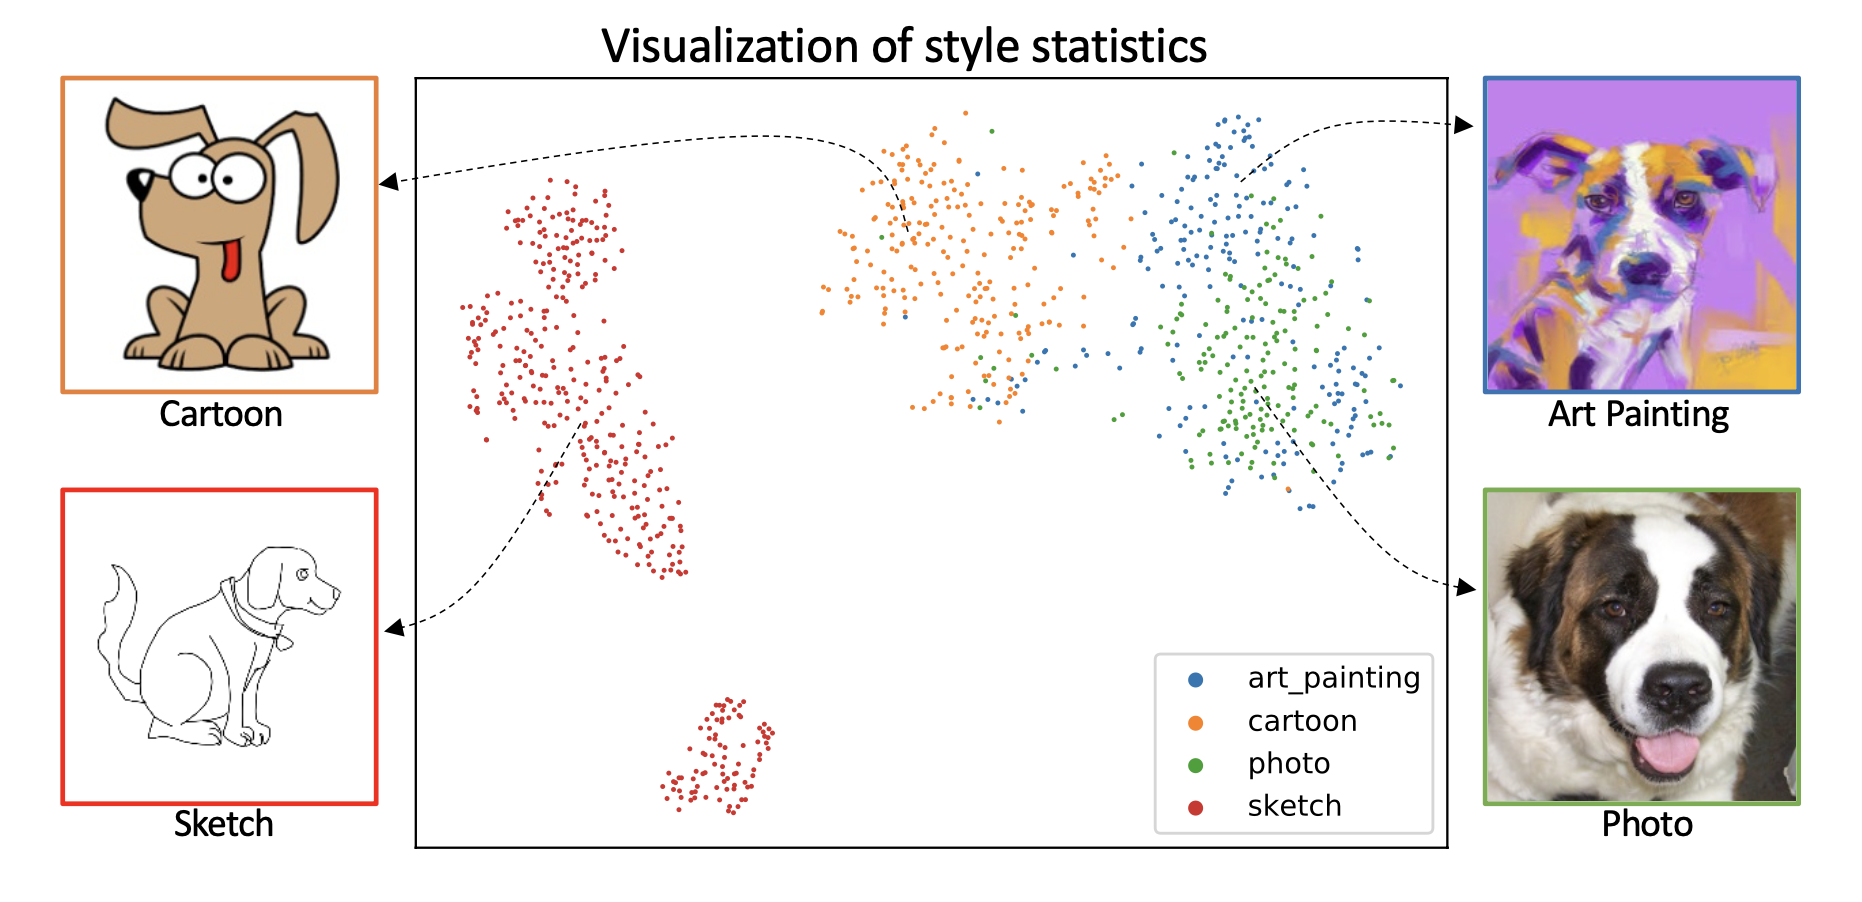
\includegraphics[width=0.5\textwidth]{images/mixstyle_domain.png}
	\caption{Cluster Overview over different domains of the same class.}
	\label{fig:mixstyle}
\end{figure}

\vspace{0.5cm}

The \textit{key idea} behind MixStyle is to simulate domain variability by mixing feature statistics - specifically, the mean and standard deviation - across different samples during training. These statistics extracted in shallow layers of the network capture style-related information, which typically varies across domains. By perturbing them in a structured manner, MixStyle implicitly encourages the network to learn representations that are invariant to style, thereby enhancing its robustness to domain shifts.

As illustrated in Figure~\ref{fig:mixstyle}, style statistics form distinct clusters for different domains. Domain generalization techniques aim to address this by reducing the separation between these clusters. The objective is to align samples of the same class, regardless of their domain origin, into a single, unified cluster. This consolidation of class-specific representations across domains leads to improved generalization and increased classification accuracy on previously unseen domains.

\subsubsection{Image Variablity}\label{susec:variability}
To modulate the degree of mixing between feature statistics from different samples, the authors utilize the $Beta$ distribution to stochastically sample a mixing coefficient denoted by $\lambda$. This coefficient controls the extent to which the style characteristics - specifically, the mean and standard deviation - of each input sample contribute to the resulting mixed representation. A value of $\lambda$ close to 0 or 1 results in an asymmetric combination, where the output is dominated by the style statistics of a single sample, with only a minimal influence from the other. Conversely, when $\lambda$ is near 0.5, the contribution from both samples becomes more balanced, yielding a more homogeneous mixture of their style attributes.

\begin{figure}[h!]
	\centering
	\begin{subfigure}[b]{0.45\textwidth}
		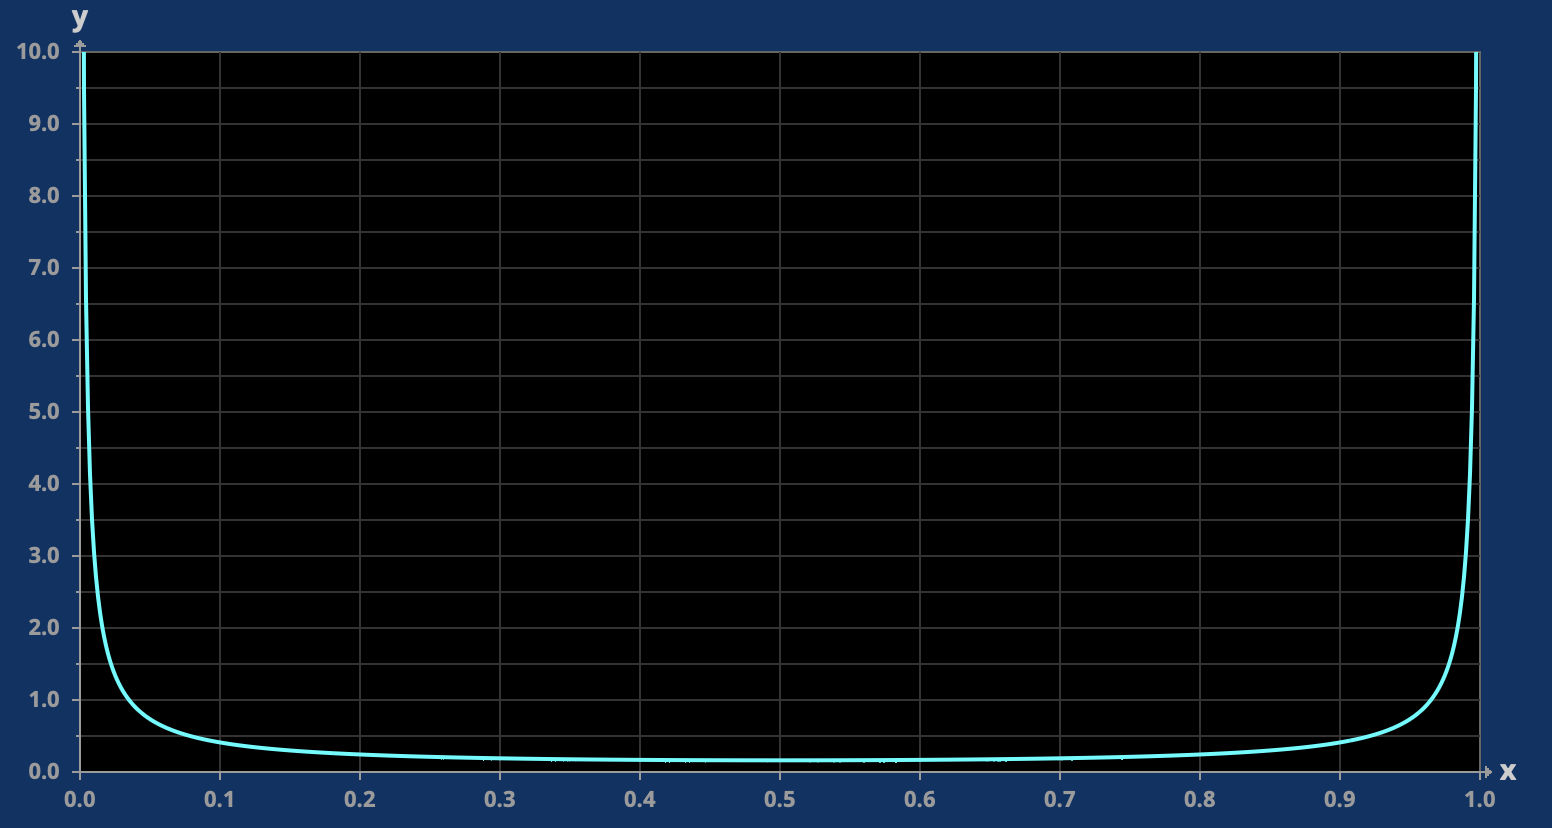
\includegraphics[width=\textwidth]{images/beta01.png}
		\caption{$\alpha = 0.1$}
		\label{fig:alpha01}
	\end{subfigure}
	\hfill
	\begin{subfigure}[b]{0.45\textwidth}
		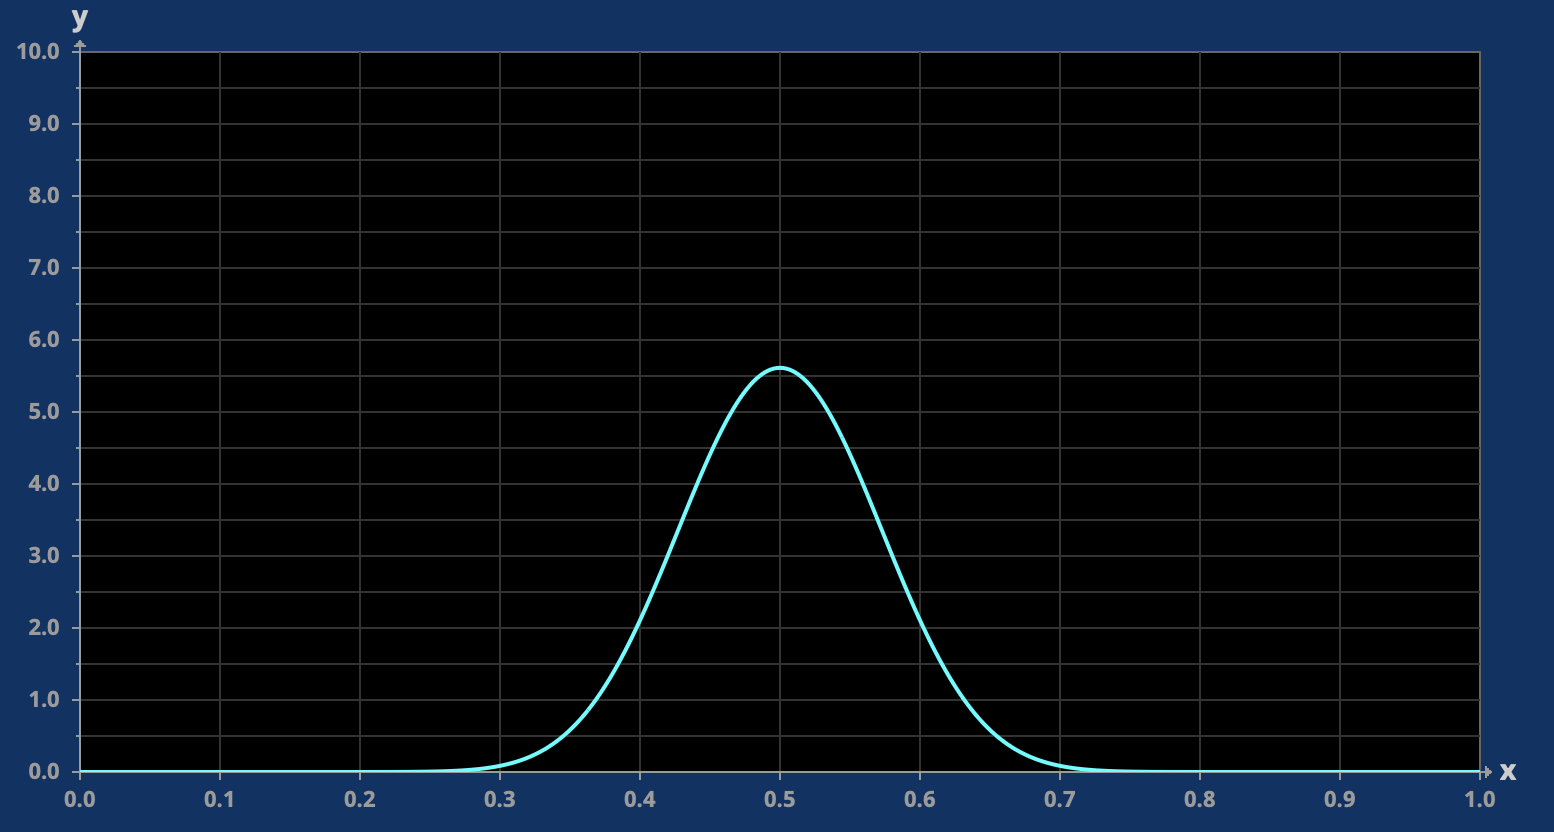
\includegraphics[width=\textwidth]{images/beta25.png}
		\caption{$\alpha = 25$}
		\label{fig:alpha25}
	\end{subfigure}
	\caption{Probability density functions of the $Beta$ distribution with symmetric parameters ($\text{$Beta$}(\alpha, \alpha)$) for different values of $\alpha$.}
	\label{fig:combined_images}
\end{figure}

The value of $\lambda$ is sampled from a symmetric $Beta$ distribution, $\text{$Beta$}(\alpha, \alpha)$, where the hyperparameter $\alpha$ determines the shape of the distribution. For small values of $\alpha$ (e.g., $\alpha = 0.1$) (as shown in Figure \ref{fig:alpha01}), the distribution is U-shaped, assigning higher probability density to values near 0 and 1. This leads to sampled $\lambda$ values that strongly favor one sample over the other, thus resulting in mixed features dominated by the style of a single image. In contrast, larger values of $\alpha$ (e.g., $\alpha = 25$) (Figure \ref{fig:alpha25}) yield a unimodal distribution centered around 0.5, promoting more balanced combinations where the styles of both samples are equally represented. This parameterization allows fine-grained control over the strength and symmetry of feature mixing.

The entire process is applied over mini-batches during training and supports two distinct strategies for selecting image pairs to be mixed. In the random sampling method, pairs of samples are selected at random from the mini-batch, without considering their domain labels. As a result, samples from the same domain may also be combined. In contrast, the cross-domain (xdomain) strategy enforces domain diversity by ensuring that each selected pair consists of samples originating from different domains. This targeted mixing encourages the model to generalize across domain boundaries by explicitly learning representations that are invariant to domain-specific style variations.

\subsubsection{Mechanism}\label{sususec:mechanismmixstyle}

\begin{algorithm}[H]\label{algorithm:mixstyle}
	\caption{MixStyle Operation Forward Pass}
	\KwIn{Feature map $\mathbf{f}$, Feature map $\mathbf{f}'$, parameter $\alpha$}
	\KwOut{Modified feature map $\hat{\mathbf{f}}$}
	Compute mean $\mu$ and std $\sigma$\;
	Sample $\lambda \sim \text{Beta}(\alpha, \alpha)$\;
	Compute mixed $\mu_c$ and $\sigma_c$\;
	Normalize and re-style\;
	\Return{$\hat{\mathbf{f}}$}
\end{algorithm}

The MixStyle layers are positioned immediately after convolutional layers, which are responsible for extracting task-relevant feature representations from the input images.

Given two feature maps, $\mathbf{f}$ and $\mathbf{f'}$, extracted from two different images (potentially from different domains), the first step involves computing the channel-wise mean and standard deviation of each feature map. These statistics are calculated over the spatial dimensions of each channel as follows:

\begin{equation}
	\mu_c = \frac{1}{HW} \sum_{h=1}^{H} \sum_{w=1}^{W} x_{c,h,w}, \qquad
	\sigma_c = \sqrt{ \frac{1}{HW} \sum_{h=1}^{H} \sum_{w=1}^{W} (x_{c,h,w} - \mu_c)^2 }
\end{equation}

Here, $x_{c,h,w}$ denotes the activation at channel $c$ and spatial location $(h, w)$, while $H$ and $W$ represent the height and width of the feature map, respectively. The computed $\mu_c$ and $\sigma_c$ describe the style characteristics of the input sample, inspired by style transfer techniques where such statistics are associated with visual appearance.

Following the computation of these style statistics, a mixing coefficient $\lambda$ is sampled from a Beta distribution, as described in Section \ref{susec:variability}. This coefficient determines the extent to which the style from one sample is combined with that of another. Specifically, $\lambda$ determines whether the resulting feature representation is a strong interpolation of both styles (when $\lambda \approx 0.5$), or largely dominated by one (when $\lambda$ is close to 0 or 1). 

\begin{equation}\label{formula:2}
	\gamma_{\text{mix}} = \lambda \, \sigma(\mathbf{f}) + (1 - \lambda) \, \sigma(\mathbf{f}') \\ ;
	\beta_{\text{mix}} = \lambda \, \mu(\mathbf{f}) + (1 - \lambda) \, \mu(\mathbf{f}') \\
\end{equation}

Equation~(\ref{formula:2}) define the computation of the mixed feature statistics used in the MixStyle transformation. Specifically, the mixed standard deviation $\gamma_{\text{mix}}$ and mixed mean $\beta_{\text{mix}}$ are obtained through a random convex combination of the channel-wise statistics from the two feature maps. 

\begin{equation}\label{formula:3}
	\hat{\mathbf{f}} = \gamma_{\text{mix}} \odot \frac{\mathbf{f} - \mu(\mathbf{f})}{\sigma(\mathbf{f})} + \beta_{\text{mix}}
\end{equation}

The final output feature map of each MixStyle layer is computed as shown in Equation~(\ref{formula:3}), where the original feature representation $\mathbf{f}$ is combined with the feature statistics - mean and standard deviation - extracted from a second, randomly selected sample. This mixing process introduces stochastic style variations during training while preserving the semantic content of the features.

The purpose of this stochasticity is to simulate domain shifts in a controlled manner, thereby forcing the model to learn representations that are invariant to domain-specific style variations. By disentangling style from content, MixStyle helps the network generalize more effectively to previously unseen domains.

\subsubsection{Benefits}
The MixStyle method demonstrates several key advantages described by \cite{mixstyle_ref} supported by extensive experimental results. First, it significantly improves domain generalization, consistently outperforming vanilla ResNet-18 and other regularization techniques on benchmark datasets. Specifically, MixStyle achieves approximately a 4\% increase in accuracy on the PACS dataset and a 1\% improvement on Office-Home compared to the traditional Mixup method. This performance gain is notable given the method’s simplicity, which also allows it to surpass more complex approaches such as L2A-OT by nearly 1\% on PACS.

MixStyle exhibits particular strength in low-data regimes, delivering over 6\% improvement with only 10 labels per class and nearly 7\% improvement with 5 labels per class on PACS, demonstrating its effectiveness in scenarios with limited training data. Additionally, the method’s versatility is evident as it achieves strong results not only in supervised learning environments but also in unsupervised and semi-supervised domain adaptation settings.

However, while MixStyle excels on smaller datasets, it does not outperform more advanced methods like L2A-OT on larger datasets such as Office-Home when applied alone, indicating opportunities for further refinement or combination with complementary techniques.

\subsubsection{Integration}
Based on the assumption that domain-related style statistics are more prominent in the shallow layers of convolutional neural networks (CNNs), MixStyle should be integrated into earlier layers of the architecture. For instance, in ResNet architectures, the optimal configuration involves inserting MixStyle behind the first and the second residual blocks. This setup enables the synthesis of "new domains" without disrupting the semantic representations required for the primary task - such as image classification - which are typically learned in deeper layers.

\cite{mixstyle_ref} recommend this configuration across different task settings. Specifically, for object recognition, they found that placing MixStyle after residual Blocks 1, 2, and 3 yields the best performance. Our setup, as detailed in Section~\ref{...}, follows a similar approach for image classification tasks. In contrast, introducing MixStyle in later layers leads to a decline in performance, likely due to the mixing of high-level semantic features, which negatively affects classification accuracy.

The implementation, as described in Section~\ref{sususec:mechanismmixstyle}, is structured around a Python module that defines the mathematical operations of MixStyle within the forward function as shown in Listing~\ref{listingMixstyle}. This design ensures that all computations are executed during the forward pass. Additionally, a new module was introduced to encapsulate the various model architectures used during training and evaluation. Within this module, a parent class was defined for each model, extended with parameters that specify the insertion points of the MixStyle layers. This modular and parameterized approach enables seamless integration of MixStyle into different architectures, making it well-suited for use during model training.

\begin{lstlisting}[language=Python, caption={MixStyle implementation structure}, label=listingMixstyle]
class MixStyle(nn.Module):
	...
	def __init__(self, p=0.5, alpha=0.1, eps=1e-6, mix="random", seed=42):
	...
	
	def forward(x):
	...
\end{lstlisting}

To support the integration of MixStyle into various model architectures, an additional module was developed to encapsulate and manage different network configurations used for training and evaluation. This module defines a parent class for each model, extended with parameters that allow precise control over the insertion points of MixStyle layers. These configurations are predefined and stored under specific model names that also encode additional details such as the position of MixStyle layers and the setup of the final classification layer.

As illustrated in Listing~\ref{listingModelLoading}, model instances can be easily loaded by referencing their respective names from the \texttt{resnet\_ms} module. This approach ensures a flexible and reproducible training pipeline, as each model variant is preconfigured with consistent parameters.

\begin{lstlisting}[language=Python, caption={Model loading from predefined configurations}, label=listingModelLoading]
	MODEL = resnet_ms.resnet50_fc512_ms12_a0d1
\end{lstlisting}

To facilitate experimental reproducibility and ease of use, the most effective architectures were encapsulated as callable model definitions. These predefined models can be conveniently loaded within Jupyter notebooks or scripts, enabling seamless execution of various training and evaluation scenarios across different configurations. 

\section{Experiments \& Results}

This section describes the conducted experiments and highlights the main results, including the most promising configurations as well as their performance. It also presents the results of two small-scale ablation studies.

\subsection{Experiments Overview}

First, we needed to establish a baseline to compare methods like MixStyle against. As mentioned previously, the two most promising backbones were ResNet-18 and ResNet-50. It is hence sensible to select their vanilla variants for this purpose. Against that baseline, we conducted three different experiments: layer freezing, MixStyle and a combination of both. Layer freezing seemed promising as the feature extraction process in the earlier layers should be no different across the domains. Freezing those layers hence could stabilize the feature extraction for the later layers to become more domain invariant. MixStyle does not need further introduction at this point and a combination of both could yield a more stable perturbation in the feature space. Among the configurations, the most notable parameters were which layers to freeze, after which layers to include a MixStyle layer and what $\alpha$ to use in the MixStyle layers.

\subsection{Effects of Configurations}

We employ freezing to enable more stable feature extraction. Freezing later layers has the consequence of reducing the model's ability to generalize to new domains. We noticed that especially freezing the last two layers decreases the performance substantially. MixStyle is also best applied in earlier layers. Perturbing the output of later layers decreases performance, as semantic information rather than style information would be mixed in doing so.

For configurations with freezing as well as with MixStyle, it has shown that introducing a 512-dimensional fully-connected layer right before the classification layer slightly increases performance. An explanation could be that as both methods make it harder or even impossible for earlier layers to adapt to the data, a fully-connected layer at the end balances the capacity of the model and introduces more learning capabilities in the latent space.

\subsection{Experimental Results}

\begin{table}[t]
    \centering
    \caption{Experimental results using three domains of PACS for training and one for validation. Results are given as mean $\pm$ standard deviation of the mean accuracy across three seeds. The accuracy is given in percent. The upper two models are our baseline, the models beneath are the different configurations from our experiments, all with ResNet-50 as backbone. FC means introducing a 512-dimensional fully connected layer after the feature maps. FR$x$ means freezing layer $x$. MS$x$ means introducing a MixStyle layer after layer $x$.}
    \label{tab:results}
    \vspace{.5em}
    \adjustbox{width=\textwidth,center}{
    \begin{tabular}{l c c c c c}
        \toprule
        \textbf{Model} & \textbf{Art painting} & \textbf{Cartoon} & \textbf{Photo} & \textbf{Sketch} & \textbf{Total} \\
        \midrule
        ResNet-18 & $78.06 \pm 0.22$ & $76.51 \pm 0.51$ & $97.94 \pm 0.28$ & $66.43 \pm 1.29$ & $77.89 \pm 0.29$ \\
        \midrule
        ResNet-50 & $84.80 \pm 0.26$ & $74.53 \pm 0.22$ & $\mathbf{98.12 \pm 0.12}$ & $68.66 \pm 1.29$ & $81.53 \pm 0.41$ \\
        + FC + FR1 & $85.24 \pm 0.58$ & $71.90 \pm 1.90$ & $\mathbf{98.12 \pm 0.16}$ & $68.84 \pm 1.02$ & $81.03 \pm 0.81$ \\
        + FC + FR1\&2 & $84.13 \pm 0.38$ & $72.45 \pm 1.15$ & $97.74 \pm 0.12$ & $70.83 \pm 0.86$ & $81.29 \pm 0.15$ \\
        + FC + MS1 & $86.98 \pm 0.69$ & $75.87 \pm 0.95$ & $\mathbf{98.00 \pm 0.22}$ & $74.13 \pm 2.24$ & $83.74 \pm 0.16$ \\
        + FC + MS1\&2 & $88.77 \pm 0.63$ & $\mathbf{76.74 \pm 1.21}$ & $\mathbf{98.18 \pm 0.07}$ & $\mathbf{75.50 \pm 1.36}$ & $\mathbf{84.80 \pm 0.05}$ \\
        + FC + FR1\&2 + MS2 & $87.61 \pm 0.53$ & $74.57 \pm 2.79$ & $\mathbf{98.28 \pm 0.03}$ & $73.79 \pm 0.90$ & $83.56 \pm 0.67$ \\
        + FC + FR1 + MS1\&2 & $\mathbf{89.11 \pm 0.29}$ & $\mathbf{76.70 \pm 0.96}$ & $\mathbf{98.10 \pm 0.06}$ & $75.14 \pm 0.75$ & $\mathbf{84.76 \pm 0.49}$ \\
        \bottomrule
    \end{tabular}}
\end{table}

The results of our baseline as well as from our most promising configurations are shown in table \ref{tab:results}. First of all, note that ResNet-50 is clearly more performant than ResNet-18. That is also the reason why the rest of the experiments use ResNet-50 as their backbone. The table also shows that freezing the first two layers doesn't seem to affect the performance. MixStyle, however, brings a substantial performance increase of about 3\%. This is also confirming the results of \cite{zhouMixStyleNeuralNetworks2023}. The most notable difference lies in the sketch domain, which is the hardest of the four. Here, MixStyle even increases performance by about 7\%. The first layer is the most important one for introducing MixStyle, as the boost in performance is most noticeable here. We had the best results with $\alpha = 0.1$, which suggests that more extreme perturbations are more effective in domain generalization. We also tested $\alpha = 0.2$ and $\alpha = 0.3$, for which the performance gradually decreased. Combining MixStyle with layer freezing does not seem to improve performance further, suggesting that MixStyle is best applied on its own.

The performance across all ResNet-50 models in the photo domain is also consistently high at about 98\%. This points out that including this domain when evaluating models pretrained on ImageNet is less informative as the domain gap is almost nonexistent compared to the other domains. A comparison with models trained from scratch would provide more insight here.

To evaluate the performance of MixStyle in the latent space, we analyzed the output of the models right before the classification layer with t-SNE. The corresponding plots of a ResNet-50 model with an introduced 512-dimensional fully-connected layer with and without MixStyle are shown in figure \ref{fig:tSNE}. For both models, sketch was used as the validation domain, hence this domain is clearly separated from the rest. Ideally, MixStyle should make the clusters more uniform, so that one class should fall in the same cluster for all domains. It is barely noticeable, but the clusters are a bit more overlapping with MixStyle. There is also more structure to the sketch cluster which indicates a slightly better separation of classes in this domain.

\begin{figure}
    \centering
    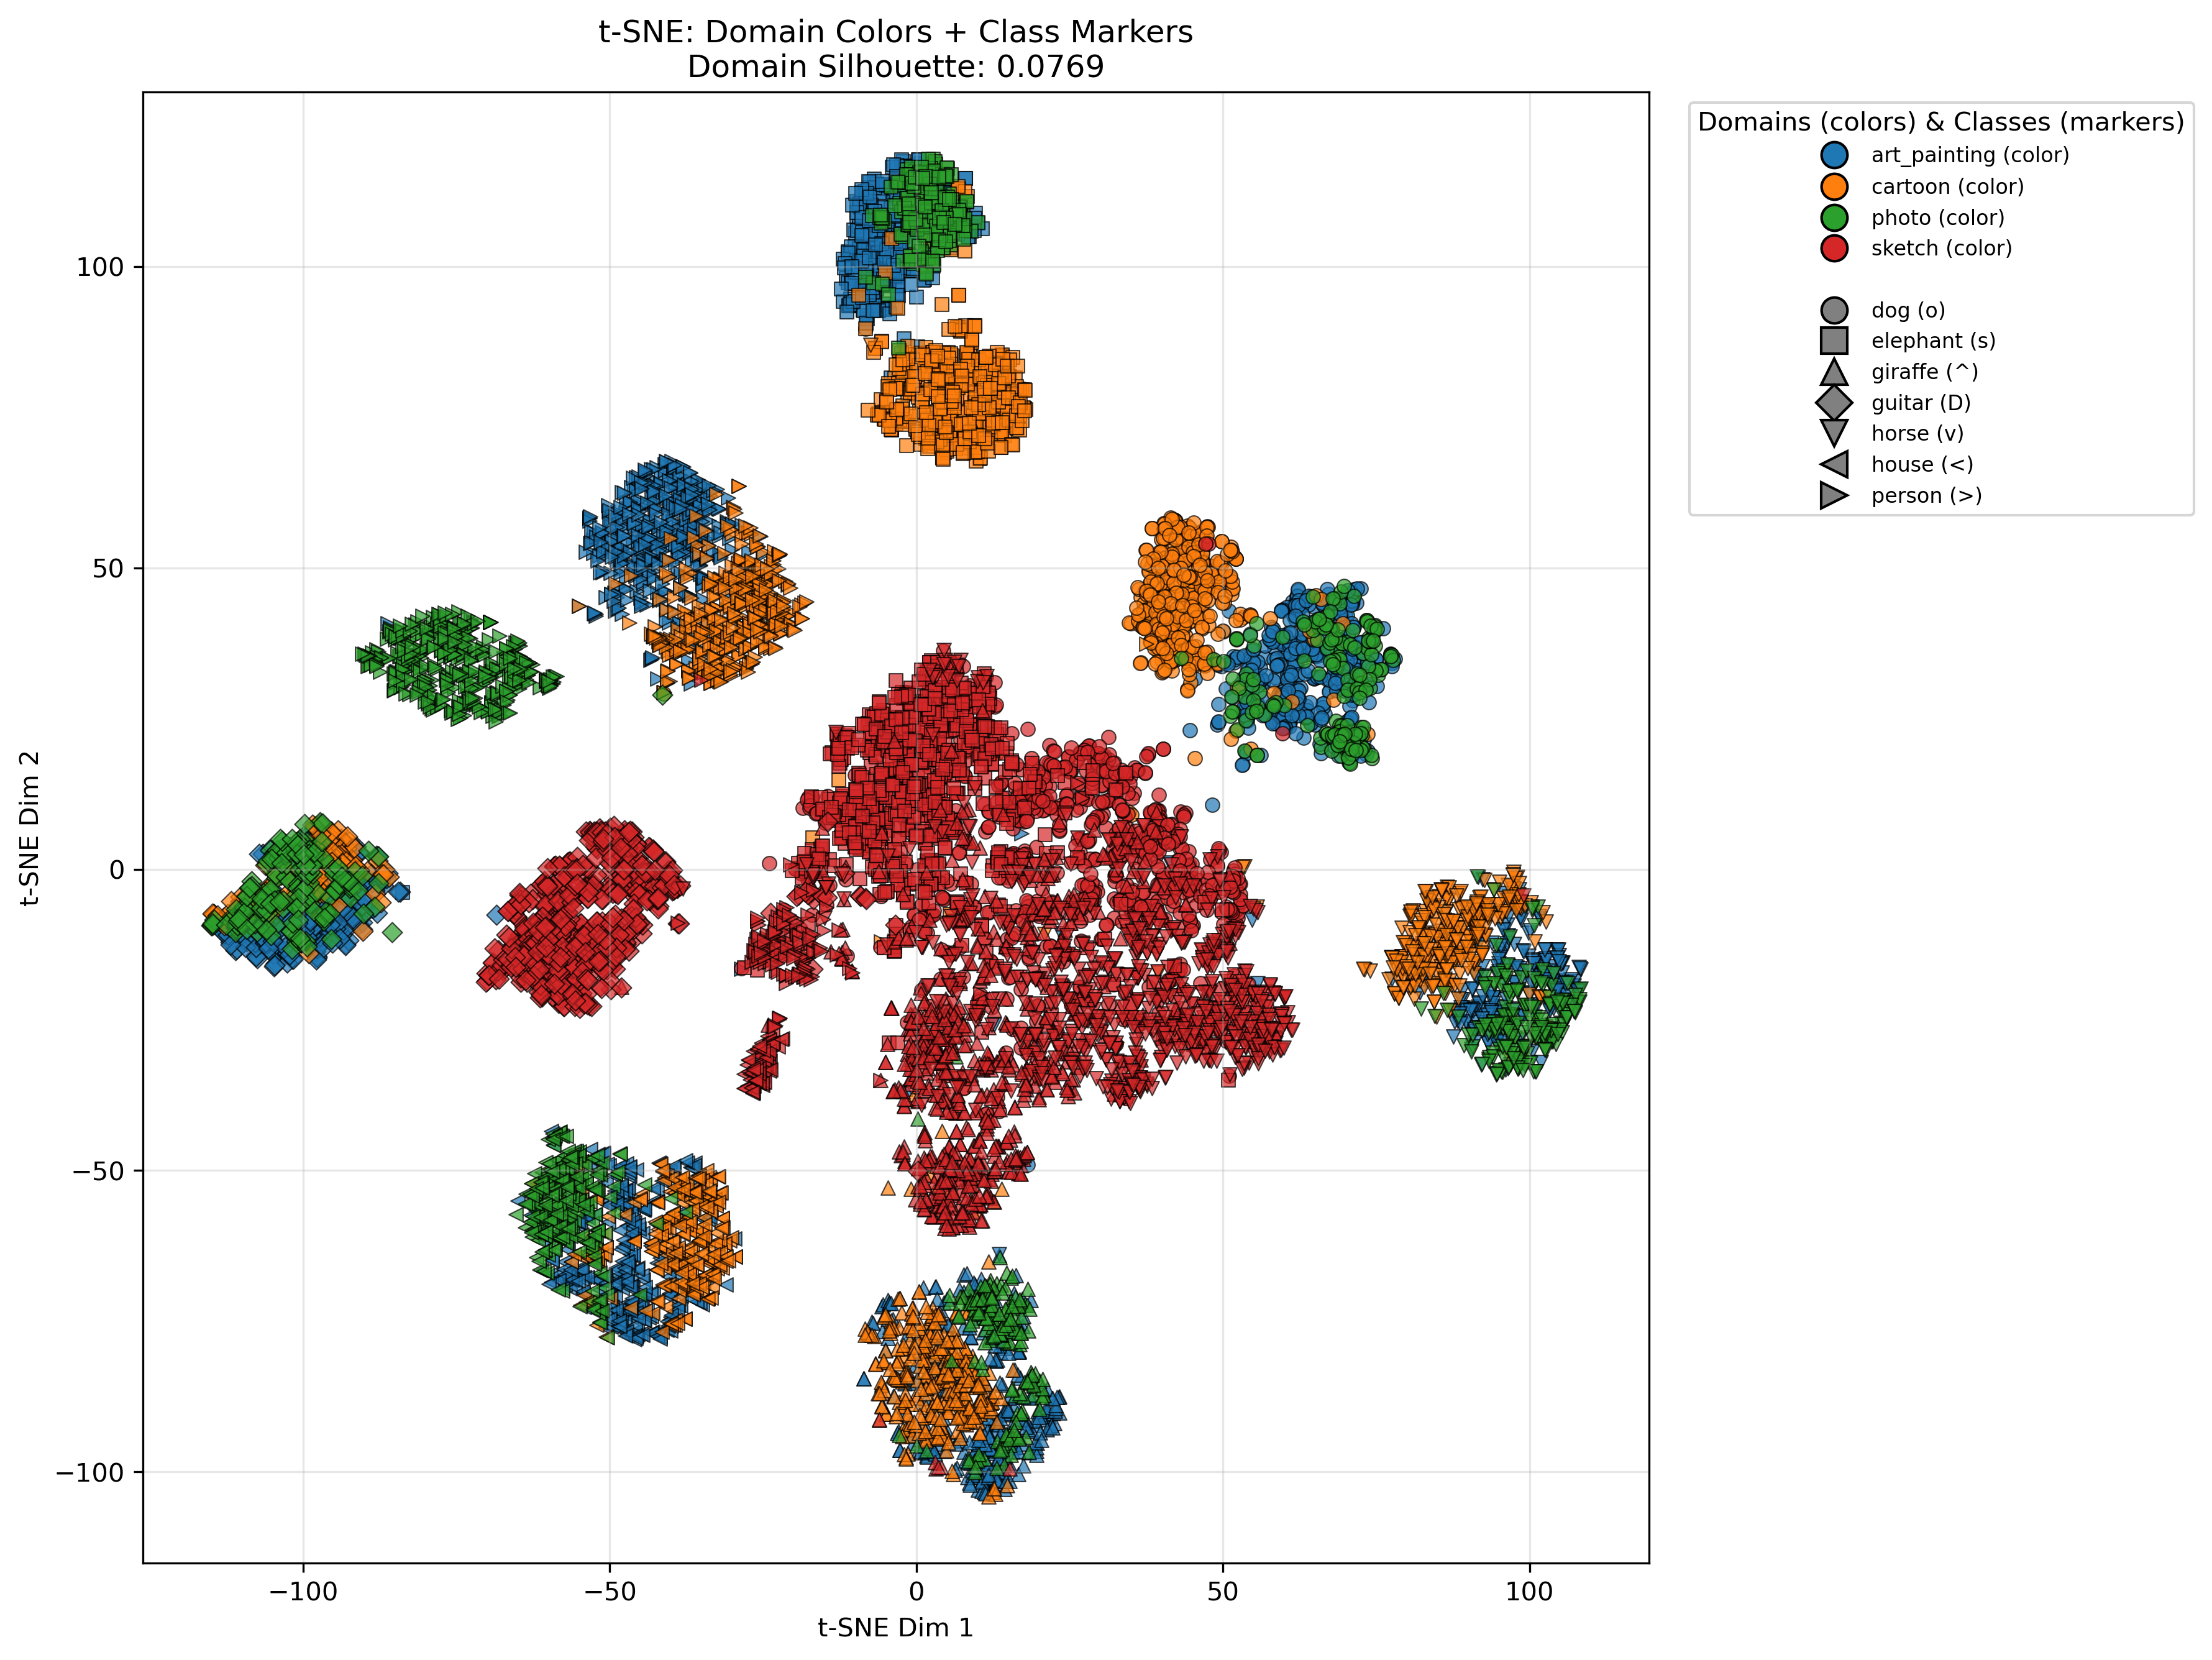
\includegraphics[width=.95\textwidth]{images/tsne_pacs_resnet50_fc512_ms12_a0d1_.png}
    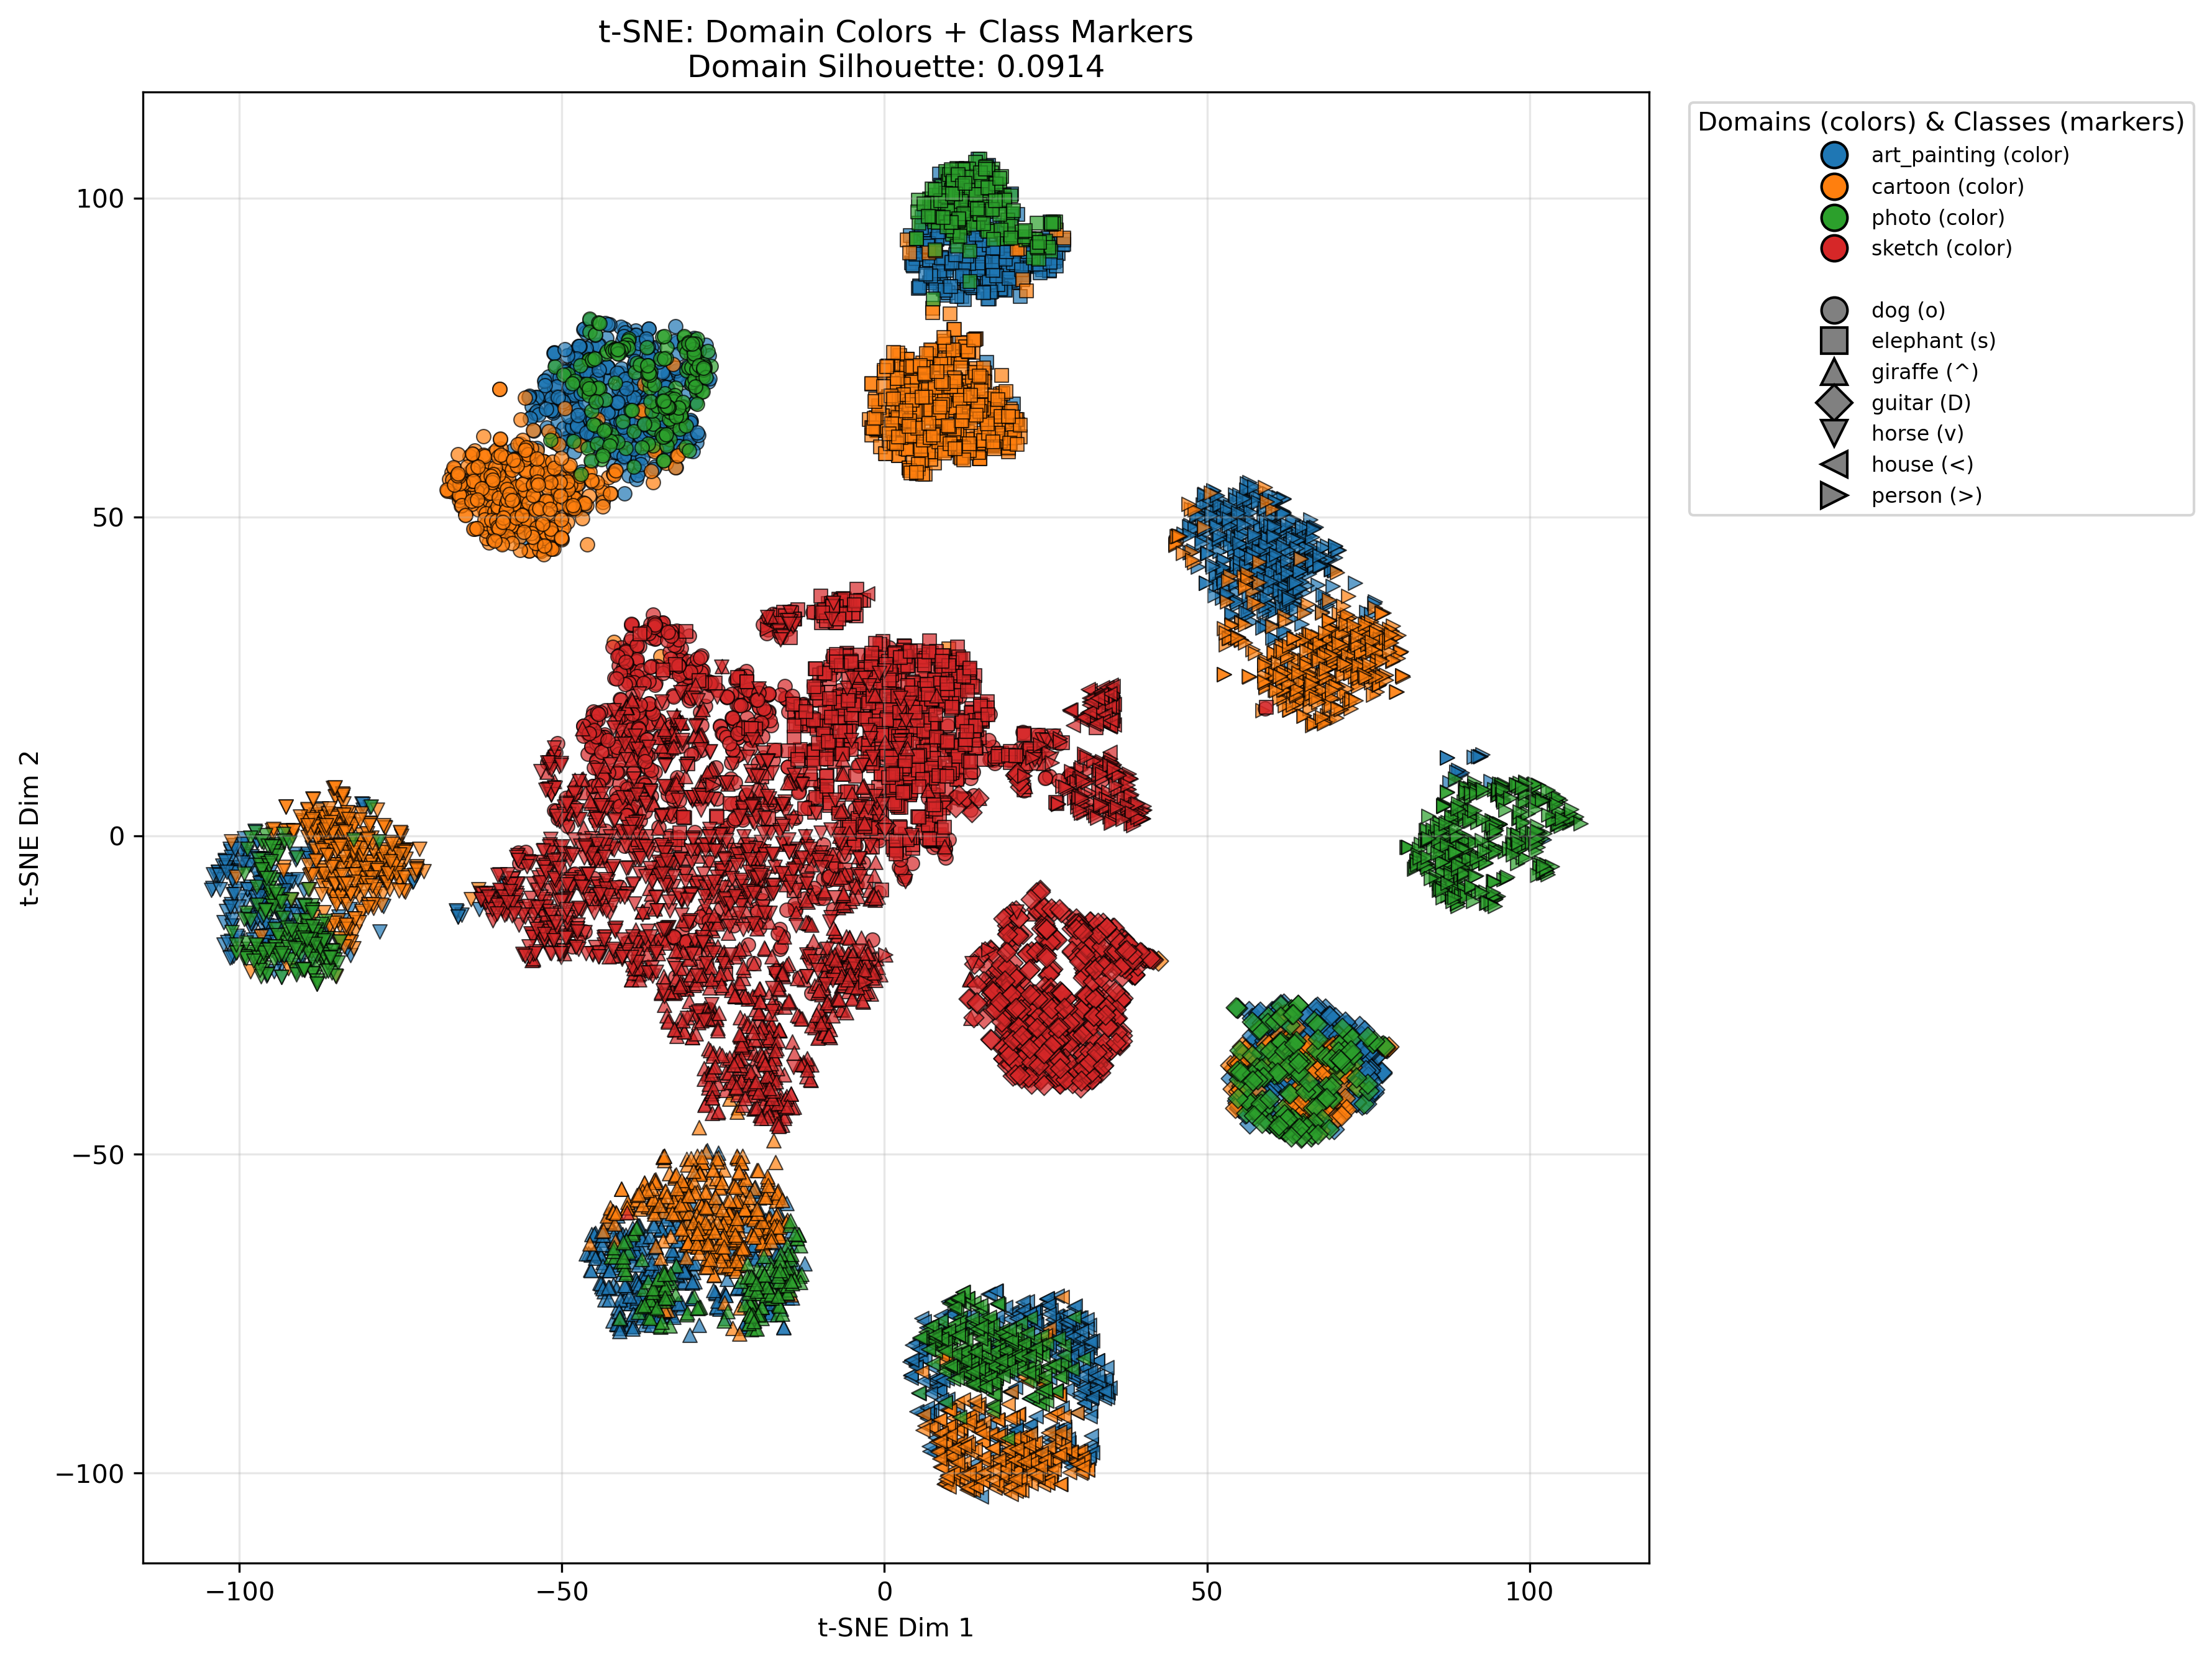
\includegraphics[width=.95\textwidth]{images/tsne_pacs_resnet50_fc512_.png}
    \caption{t-SNE evaluation from the output of an introduced 512-dimensional fully connected layer right before the classification layer of a ResNet-50 model with (top) and without (bottom) MixStyle after the first two layers, respectively. For both models, sketch (red) was used as validation domain.}
    \label{fig:tSNE}
\end{figure}

\subsection{Ablation Studies}

\begin{table}[t]
    \centering
    \begin{minipage}[t]{0.48\textwidth}
        \centering
        \caption{Results of an ablation study on a threefold split of PACS into train, validation and test set. Results are given as mean $\pm$ standard deviation of percent accuracy. The model used was ResNet-50 + FC + MS1\&2 + FR1.}
        \label{tab:results_threefold}
        \vspace{.5em}
        \begin{tabular}{l c}
            \toprule
            Art painting & $73.08 \pm 4.52$ \\
            Cartoon & $74.69 \pm 0.26$ \\
            Photo & $97.32 \pm 0.15$ \\
            Sketch & $70.54 \pm 2.95$ \\
            \midrule
            Total & $78.90 \pm 1.70$ \\
            \bottomrule
        \end{tabular}
    \end{minipage}
    \hfill
    \begin{minipage}[t]{0.48\textwidth}
        \centering
        \caption{Results of one run on Office-Home with the model ResNet-50 + FC + MS1\&2. Due to computational time constraints, only one run was evaluated. Results are given as percent accuracy.}
        \label{tab:results_office-home}
        \vspace{.5em}
        \begin{tabular}{l c}
            \toprule
            Art & $63.29$ \\
            Clip art & $48.74$ \\
            Product & $73.89$ \\
            Real World & $76.29$ \\
            \midrule
            Total & $65.55$ \\
            \bottomrule
        \end{tabular}
    \end{minipage}
\end{table}

In a first ablation study, we split the dataset into three parts. One domain was used for validation, one for testing and two for training. We iterated through the domains to select a test domain. The validation domain was chosen among the remaining domains at random. The results are shown in table \ref{tab:results_threefold}. This experiment is again a great illustration that the photo domain brings no insight because of the use of pretrained weights. It is however interesting to see that the other three domains have much more similar performance than in the twofold split.

We additionally evaluated one model on the Office-Home dataset. Due to computational time constraints, we were only able to run one seed as that takes about 7 hours on our hardware to complete. Table \ref{tab:results_office-home} lists the results. Office-Home has 65 classes, so a worse performance than on PACS was to be expected. Overall, the accuracy here remains high, supporting the results of \cite{zhouMixStyleNeuralNetworks2023}.

\section{Discussion}

As described in the previous section, freezing early layers doesn't seem to affect the performance at all. This suggests that the feature extractors in the earlier layers are quite stable even without freezing across the domains, which is plausible, as basic shapes and low-level features remain consistent across different domains.

Mixstyle on the other hand is a very promising technique, which has shown to enable great performance increases. Our results demonstrate that Mixstyle is best applied after the first two layers, with the most important layer being the first one. This makes sense as basic shapes and style information are conveyed at this stage. A perturbation at this level is hence the most effective for domain generalization. Our experiments also show that a smaller $\alpha$, i.e., a more extreme perturbation, is more effective. By introducing artificial domains with heavier stylistic changes less frequently, the model sees more variety in domains during training while still having information of the original domains. This results in a better ability to generalize across domains.

Our results also show a flaw in the experimental setup, including that commonly used in the field. Using pretrained weights is problematic as certain domains essentially become irrelevant. Prime examples for that are the ``photo'' domain in PACS as well as the ``product'' and ``real world'' domains from Office-Home. In the latter case, even two domains are affected by data leakage. This suggests that results are better gathered by not using pretrained weights when just assessing the performance of domain generalization techniques. In practice, however, pretrained weights are often beneficial, which creates a tension that warrants further investigation.

The datasets used in our study also have limitations that should be acknowledged. PACS and Office-Home represent relatively controlled scenarios with clearly defined domain boundaries. Real-world domain shifts are often more subtle and continuous, and it is unclear whether more gradual style shifts affect the effectiveness of Mixstyle. Additionally, while our tSNE analysis shows some improvement in feature clustering, the differences are quite subtle and could benefit from more detailed analysis.

Overall, looking back at the results, Mixstyle is a lightweight, parameter-free and highly effective method for domain generalization. The technique shows consistent improvements across different domains, with particularly strong gains in challenging domains like sketch. However, it is important to mention that the datasets used in our study represent controlled scenarios, and future work should investigate how well these findings transfer to more naturalistic domain shifts encountered in practical applications.
\section{Conclusion}


\section{Notation}
% SOURCE: https://github.com/goodfeli/dlbook_notation/blob/master/math_commands.tex
% Quote from github "We make them freely available for anyone to use."


% Sometimes we have to include the following line to get this section
% included in the Table of Contents despite being a chapter*
This section provides a concise reference describing notation as used in the book by \citet{goodfellow2016deep}.
If you are unfamiliar with any of the corresponding mathematical concepts,
\citet{goodfellow2016deep} describe most of these ideas in
chapters 2--4. \\[0.7cm]

% Need to use minipage to keep title of table on same page as table
% This is a hack to put a little title over the table
% We cannot use "\section*", etc., they appear in the table of contents.
% tocdepth does not work on this chapter.
\centerline{\bf Numbers and Arrays}
\bgroup
% The \arraystretch definition here increases the space between rows in the table,
% so that \displaystyle math has more vertical space.
\def\arraystretch{1.5}
\begin{tabular}{cp{3.25in}}
$\displaystyle a$ & A scalar (integer or real)\\
$\displaystyle \va$ & A vector\\
$\displaystyle \mA$ & A matrix\\
$\displaystyle \tA$ & A tensor\\
$\displaystyle \mI_n$ & Identity matrix with $n$ rows and $n$ columns\\
$\displaystyle \mI$ & Identity matrix with dimensionality implied by context\\
$\displaystyle \ve^{(i)}$ & Standard basis vector $[0,\dots,0,1,0,\dots,0]$ with a 1 at position $i$\\
$\displaystyle \text{diag}(\va)$ & A square, diagonal matrix with diagonal entries given by $\va$\\
$\displaystyle \ra$ & A scalar random variable\\
$\displaystyle \rva$ & A vector-valued random variable\\
$\displaystyle \rmA$ & A matrix-valued random variable\\
\end{tabular}

\clearpage


\section*{References}

Any choice of citation style is acceptable as long as you are
consistent. It is permissible to reduce the font size to \verb+small+ (9 point)
when listing the references.
Note that the Reference section does not count towards the page limit.
\medskip


\bibliography{bibliography}
\bibliographystyle{abbrvnat}


%%%%%%%%%%%%%%%%%%%%%%%%%%%%%%%%%%%%%%%%%%%%%%%%%%%%%%%%%%%%%%%%%%%%%%%%%%%%%%%%%%%%%%%%%%%%%%%%%%%%
%% Declaration of Authorship
%%%%%%%%%%%%%%%%%%%%%%%%%%%%%%%%%%%%%%%%%%%%%%%%%%%%%%%%%%%%%%%%%%%%%%%%%%%%%%%%%%%%%%%%%%%%%%%%%%%%

\section*{Declaration of Authorship}
All final papers have to include the following ‘Declaration of Authorship’:

{\parindent 0cm
%%%%%%%%%%%%%%%%%%%%%%%%%%German%%%%%%%%%%%%%%%%%%%%%%%%%%%%%%
\section*{Declaration of Authorship}
Ich erkläre hiermit gemäß § 9 Abs. 12 APO, dass ich die vorstehende Seminararbeit selbstständig verfasst und keine anderen als die angegebenen Quellen und Hilfsmittel benutzt habe. Des Weiteren erkläre ich, dass die digitale Fassung der gedruckten Ausfertigung der Seminararbeit ausnahmslos in Inhalt und Wortlaut entspricht und zur Kenntnis genommen wurde, dass diese digitale Fassung einer durch Software unterstützten, anonymisierten Prüfung auf Plagiate unterzogen werden kann.\\
\vspace{2\baselineskip}
  
Bamberg, \today

\rule[0.5em]{14em}{0.5pt} \hspace{0.25\linewidth}\rule[0.5em]{14em}{0.5pt}
\vspace{1em}
\hspace{4em} (Ort, Datum) \hspace{0.51\linewidth} (Unterschrift)
}



%%%%%%%%%%%%%%%%%%%%%%%%%%%%%%%%%%%%%%%%%%%%%%%%%%%%%%%%%%%%


%%%%%%%%%%%%%%%%%%%%%%%%%%%%%%%%%%%%%%%%%%%%%%%%%%%%%%%%%%%%


\appendix


\section{Appendix}


Optionally include extra information (complete proofs, additional experiments and plots) in the appendix.
This section will often be part of the supplemental material.


\end{document}
